\section{Experiments}
    In this section, we analyze the performance of our model on public violence detection datasets. Our model outperforms the previous models and achieves state-of-the-art accuracy in spite of having low computational complexity and less memory footprint.

    \subsection{Datasets}
    We used three benchmark violence detection datasets for training and validating our model, namely  RWF-200 violence dataset~\cite{cheng2019rwf}, Hockey-fight dataset~\cite{hockey_nievas2011violence} and Movies-Fight dataset~\cite{movie_nievas2011violence}. 
    At the moment, the RWF-2000 violence dataset is the largest dataset for violence detection with 2000 clips. 1600 clips out are kept for training and 400 are used for validation. The clips from the dataset are collected from real-world surveillance cameras. The number of characters in the clips are not fixed, dynamic characteristics vary a lot and the background is complicated.
    Hockey-fight dataset is collected from video footage of hockey games. There are 1000 clips in the dataset, where half of them are violent and the rest are non-violent. Movies-fight dataset consists of clips from movies with a total of 200 clips. 
    
    \begin{figure*}[]
	\centering
	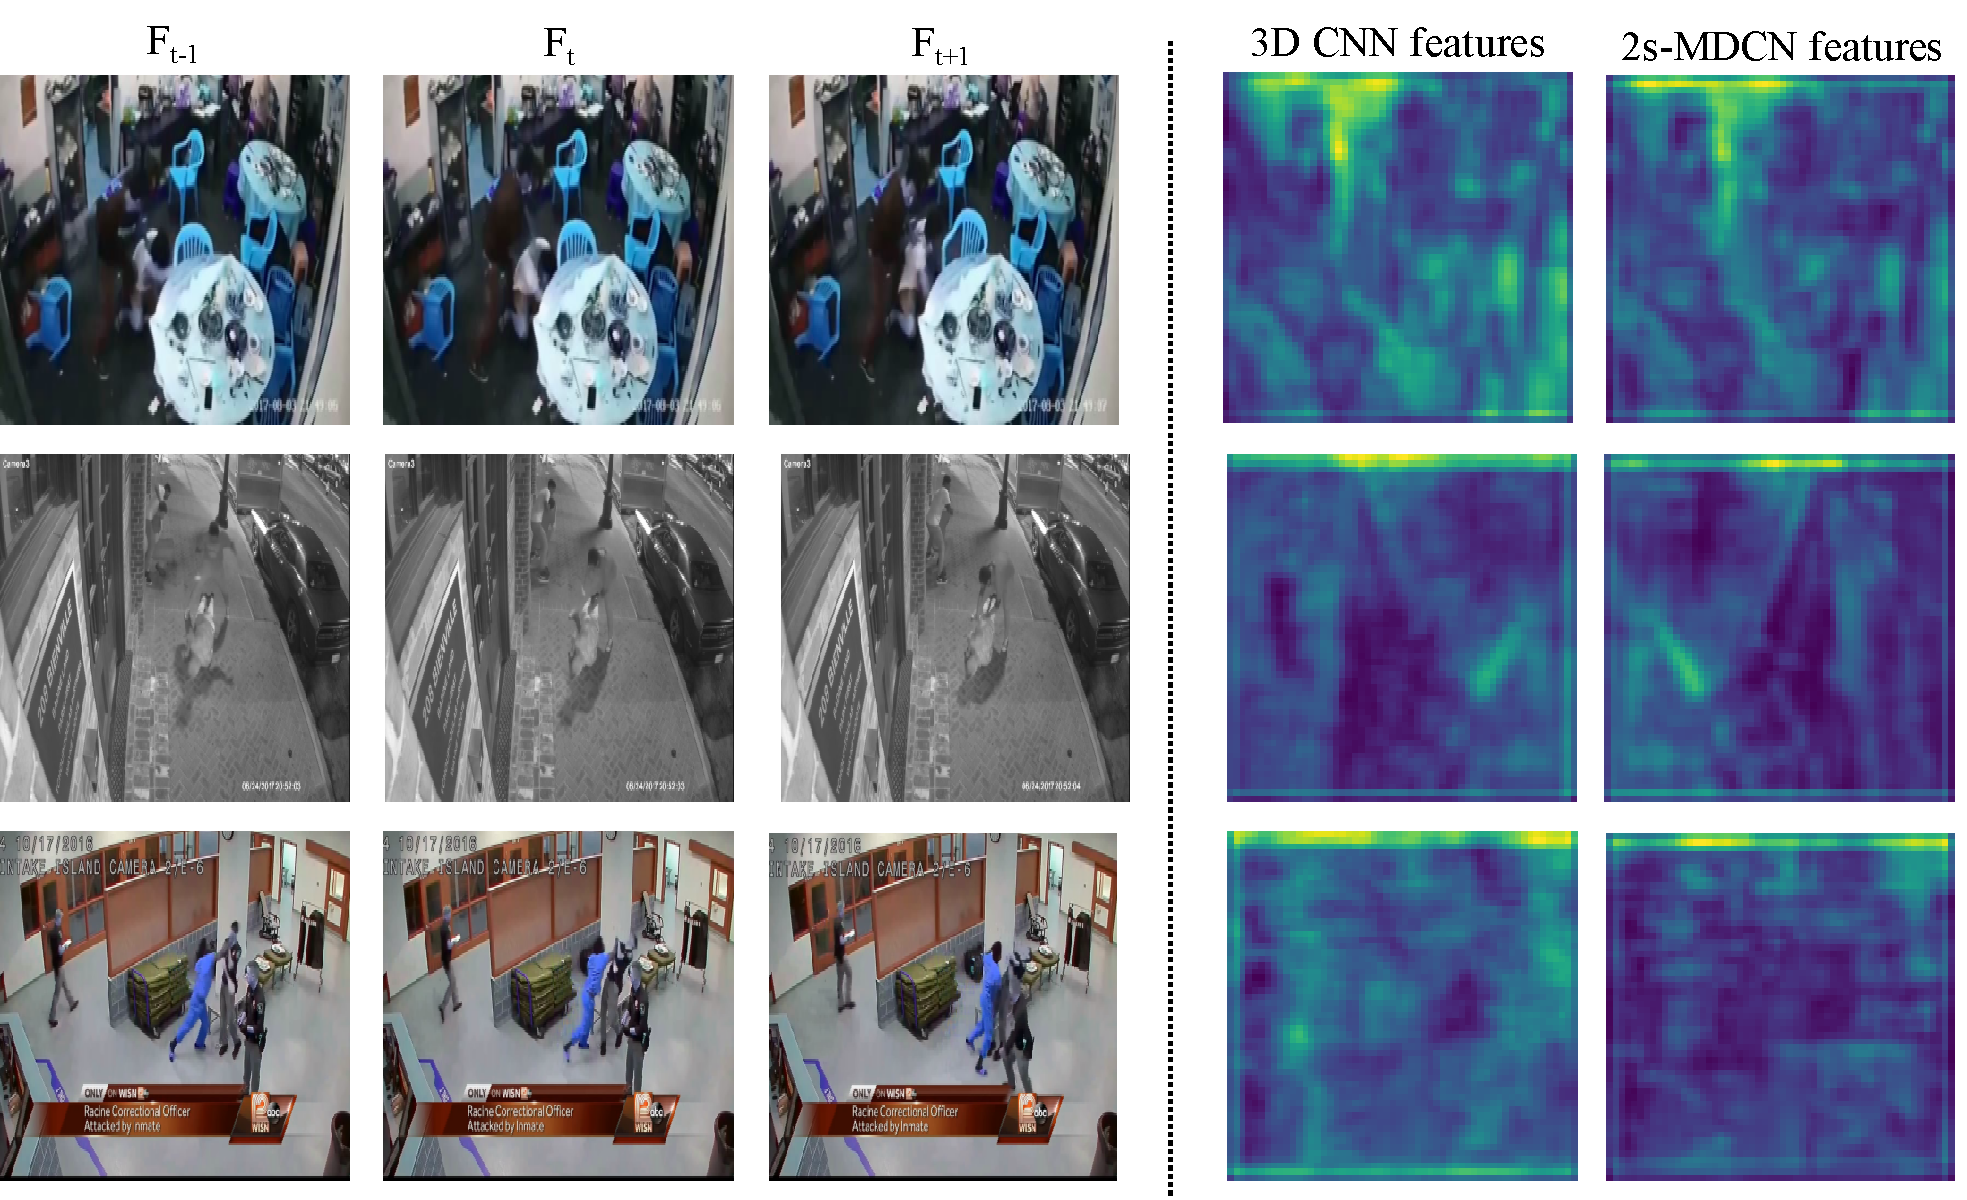
\includegraphics[width=0.9\linewidth]{new_images/features.pdf}
	\caption{Visualization of extracted features from 2s-MDCN.}
	\label{fig:features_vis}
	\end{figure*}

    \subsection{Training details}
     For training, we sampled $32$ frames from each clip and each frame was resized to ${224}\times{224}$. 
     Thus, our input size for the was ${3}\times{32}\times{224}\times{224}$. 
     Following the procedure of~\cite{cheng2019rwf}, we used brightness transformation and random rotation to augment our data in order to prevent overfitting.
     We implemented our model by using PyTorch~\cite{pytorchpaszke2019} which is a deep-learning framework. Stochastic gradient descent (SGD) optimizer was used to train our network with nesterov momentum~\cite{nesterovbotev2017} of value $0.9$. The value of weight decay was set to ${1e}^{-3}$. The initial learning rate was set to $0.1$, which was reduced by a factor of $10$ after $25$ and $75$ epochs. We trained our model for $100$ epochs with a batch size of $16$. 
%	 Violence detection is more data-driven than general human action recognition, as violence detection involves more movement, more than one character involvement, more variation of dynamic of characters.     
     Our model was trained from scratch with the corresponding datasets.
     
%     	\begin{figure}[!htb]
% 	\centering
% 	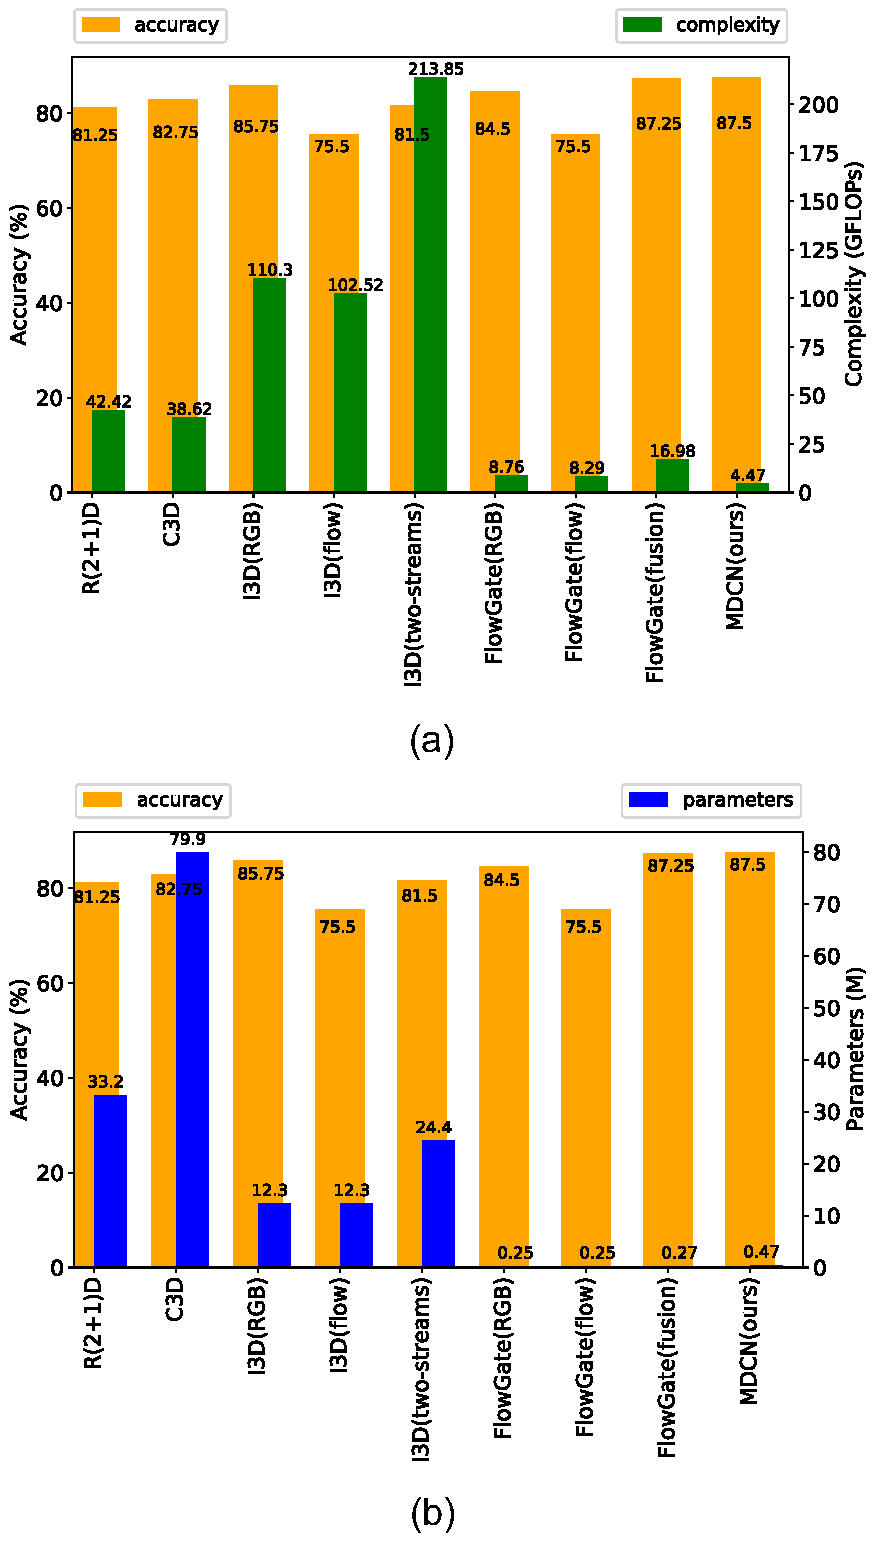
\includegraphics[width=0.9\linewidth]{mdcn/new_images/vio_result_pdf2.pdf}
% 	\caption{This figure illustrates comparison between our model and other state-of-the-art models. (a) shows the bar graph of accuracy vs. computational complexity and (b) displays the same for accurcy vs. number of parameter.}
% 	\label{fig:result_comparison}
% 	\end{figure}


%  Ablation study for skip connection  %

% 	% 	%		%		%		% 	% 	%		%		%		%
